%% skeleton.tex                 %% 12 February 2006
%% Use this file to start your paper for the UJM/18.096

\documentclass[11pt]{article}   %% Standard LaTeX.
\usepackage{amsmath,amssymb}    %% For better support of math
                                %% amssymb provides \mathbb and \square
                                
\usepackage{xcolor}
%% \usepackage{url}             %% Supports formating URLs.
%% \usepackage{graphicx}        %% Enable for eps figures

\newcommand\note[1]{\textcolor{red}{#1}}
\newcommand\PP{\mathbb{P}}
\newcommand\seq{\textsc{seq}_l}
\newcommand{\qed}{\hfill \ensuremath{\Box}}

\textwidth=6.8in
\textheight=8in
\hoffset=-0.85in
\topmargin=0.5in
\setlength{\topmargin}{0in}
\usepackage{ntheorem}
\usepackage{graphicx}

\theoremstyle{plain}
\theorembodyfont{}
\theoremsymbol{}
\theoremprework{}
\theorempostwork{}
\theoremseparator{.}

\newtheorem{theorem}{Theorem}[section]
\newtheorem{lemma}[theorem]{Lemma}
\newtheorem{proposition}[theorem]{Proposition}
\newtheorem{corollary}[theorem]{Corollary}

\newenvironment{proof}[1][Proof.]{\begin{trivlist}
\item[\hskip \labelsep {\bfseries #1}]}{\end{trivlist}}
\newenvironment{definition}[1][Definition.]{\begin{trivlist}
\item[\hskip \labelsep {\bfseries #1}]}{\end{trivlist}}
\newenvironment{example}[1][Example.]{\begin{trivlist}
\item[\hskip \labelsep {\bfseries #1}]}{\end{trivlist}}
\newenvironment{remark}[1][Remark.]{\begin{trivlist}
\item[\hskip \labelsep {\bfseries #1}]}{\end{trivlist}}
\newcommand\numberthis{\addtocounter{equation}{1}\tag{\theequation}}

\begin{document}
\pagestyle{myheadings}          %% Supports custom headers.
\markboth{\sc 6.867 - Homework 1}{\sc
6.867 - Homework 1}                  %% Running right header
\title{6.867 - Homework 1}           %% For first page
\author{Akhil Raju and Matthew Arbesfeld}
\date{September 28, 2014}         %% Change \today to draft date if you want
\maketitle
\textbf{XXX fix figure links}

\section{Implementing Gradient Descent}

\subsection{Background}
Gradient descent is a common numerical method for finding local minima or maxima in a given function. Given a starting point on the function, we follow the gradient towards local extrema. The iterative process for finding a local minimum can be described by the following equation: \[\theta_{k+1} = \theta_k - \gamma \nabla F(\theta_k)\] where $\gamma$ is the step size. The process ends when $|F(\theta_{k+1}) - F(\theta)|$ falls below some threshold convergence criterion $c$. 

\subsection{Choice of Parameters}

The choice of which starting point $\theta_0$, step size $\gamma$, and convergence threshold $c$ greatly affect the behavior of gradient descent. 

The effect of $\theta_0$ is most apparent for a non-convex function with multiple minima. Take $F(x) = \sum\limits_{i=1}^{2} {x_i}^4 - {x_i}^3 - {x_i}^2 + x_i$. $F$ has 4 different local minima. As shown in Figure \ref{initial_guesses}, the choice of our starting guess $\theta_0$ affects which of these minima our gradient descent converges to. Clearly, our choice of $\theta_0$ biases our solution towards points close to our starting guess. For a convex function, this is less problematic because we are only concerned with one minimum, but with non-convex functions, our starting guess might cause our descent to converge on a local minimum instead of the global minimum.

\begin{figure}[h!]\label{initial_guesses}
  \caption{Modifying the initial guess for gradient descent can result in different solutions for functions with multiple minima. The different colored regions converge to different local minima of $F$ (denoted in red). }
  \centering
    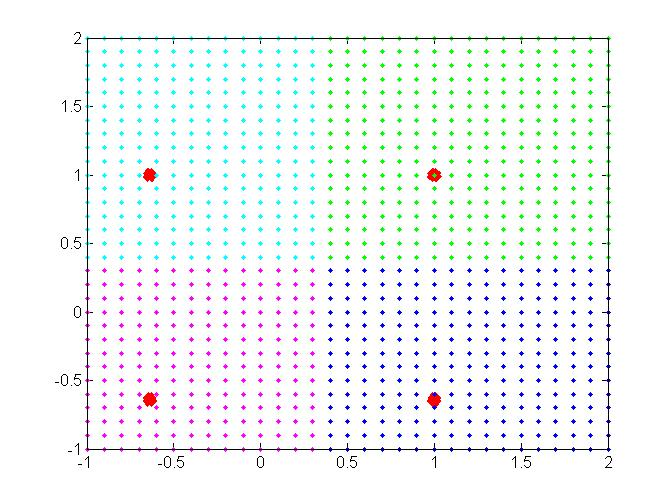
\includegraphics[width=0.5\textwidth]{figures/1_2_start_guesses.jpg}
\end{figure}

Step size has a significant effect for gradient descent on both non-convex and convex solution. In general, step size represents a trade-off between computation efficiency and accuracy of output. With a smaller step-size, we can attain a more precise minimum, but it takes more iterations to get there. Take the quadratic bowl, $Q(x,y) = X^2 + y^2$ as an example. If we start at $\theta_0 = (1,1)$ with $\gamma = 0.01$, we converge to $x_{min} \approx (0,0)$ in about 500 steps. With $\gamma = 0.1$, we converge to the same answer in about 60 steps. There is a limit to how much we can increase the step size though. In our quadratic bowl example, if we increase $\gamma = 1$, then gradient descent fails to converge on any minimum. It actually oscillates back and forth over the minimum at $x = (0,0)$ and never reaches it. Thus, if we use a fixed value for $\gamma$, we need to do so carefully. There are ways to dynamically choose a value of $\gamma$ on each step, namely a procedure called line search, but that is beyond the scope of this paper.

The convergence threshold has a similar effect on gradient descent as the step size in that it represents a trade-off between computational efficiency and precision. With a greater threshold, we take less time to converge, but the solution is farther from the actual minimum. For example, for our non-convex function $F$, if we use $\gamma = 0.1$,  $\theta_0 = (2,0)$, and $c = 0.00001$, then we converge to $x_{min} = (-0.64,-0.64)$ in 18 steps. When we change to $c = 0.001$, we converge to $x_{min} = (-0.54,-0.64)$ in 12 steps. We saved 33 percent of our work at the cost of a less precise answer.

\subsection{Numerical vs. Analytical Gradient Calculations}
We can also compute the gradient of our function numerically using central finite differences. While this approach works well for functions whose slope is slow-varying, it breaks down for functions that have quickly varying gradients. The quadratic bowl function from above, $G$, has a relatively slow-varying gradient. Thus, when the gradient is computed numerically at various points, the numerical gradient does not differ from the actual gradient. The function $F$ from above, however, does has a quickly varying gradient, and for most points close to the origin, where the gradient is most variable, the numerical gradient differs significantly from the actual gradient. 

It should be noted that the differences between the analytical (actual) gradient and the numerically calculated gradient depends heavily on the step size we choose for our calculations, a smaller value yielding a more accurate gradient.

\subsection{Comparing to Matlab}
In general, the built-in Matlab function for function minimization, fminunc(), outperforms our gradient descent procedure. For comparable accuracy, fminunc uses about 10\% to 20\% of the function calls that our gradient descent procedure requires when computing the local minimum for our non-convex function $F$.

\section{Linear Basis Function Regression}\label{sec-basis}
In this problem, we are asked to solve a linear regression problem in two ways. First, we use the analytic solution for linear regression to determine the maximum likelihood weight vector in a variety of feature spaces. We then use the gradient descent approach from Problem~\ref{sec-gradient-descent} to determine approximate solutions for each set of features. We compare the two algorithms by using sum-squared error as a metric.
\subsection{Analytic Solution}
Our data set consists of 10 points generated from the function $\sin(2 \pi x)$. We  use the analytic solution of linear regression to find the optimal weight vector of the 10 points. \\
\\
\indent Given a data set of $n$ points $\{ x^{(1)}, y^{(1)} \}, \{ x^{(2)}, y^{(2)} \}, \ldots, \{ x^{(n)}, y^{(n)} \}$ and a set of $D$ features $\phi_1, \phi_2, \ldots \phi_D$, we can construct a \textit{data matrix} \textbf{X} by applying the feature functions to every data point: \\
	 \[ \textbf{X} = \left( \begin{array}{ccccc}
1 & \phi_1(x^{(1)}) & \phi_2(x^{(1)}) & ... & \phi_D(x^{(1)}) \\
1 & \phi_1(x^{(2)}) & \phi_2(x^{(2)}) & ... & \phi_D(x^{(2)}) \\
& ......... \\
1 & \phi_1(x^{(n)}) & \phi_2(x^{(n)}) & ... & \phi_D(x^{(n)}) \end{array} \right)\] 
With sum-squared distance as our error metric, we choose a weight vector $W$ that minimizes $(\textbf{X}W - Y)^\textnormal{T} (\textbf{X}W - Y)$. Setting the derivative of this expression with respect to $W$ equal to 0 and then solving for $W$ yields an exact solution:
\begin{equation} \label{eq-analytic}
	W = (\textbf{X}^\textnormal{T}\textbf{X})^{-1}\textbf{X}^{\textnormal{T}}Y
\end{equation}
\indent With the simple feature set of polynomial basis $\phi_1(x) = x,\ldots,\phi_D(x) = x^D$, we get the solutions as shown in Figure~\ref{fig-analytic}. As $D$ increases, the sum-squared error decreases, but we can clearly see that the solution is over-fitting to the data. $D \approx 3$ produced the most accurate representation of the underlying generator function. 
\begin{figure}[h!]\label{fig-analytic}
  \caption{Analytic linear regression solution for simple polynomial basis of various sizes.}
  \centering
    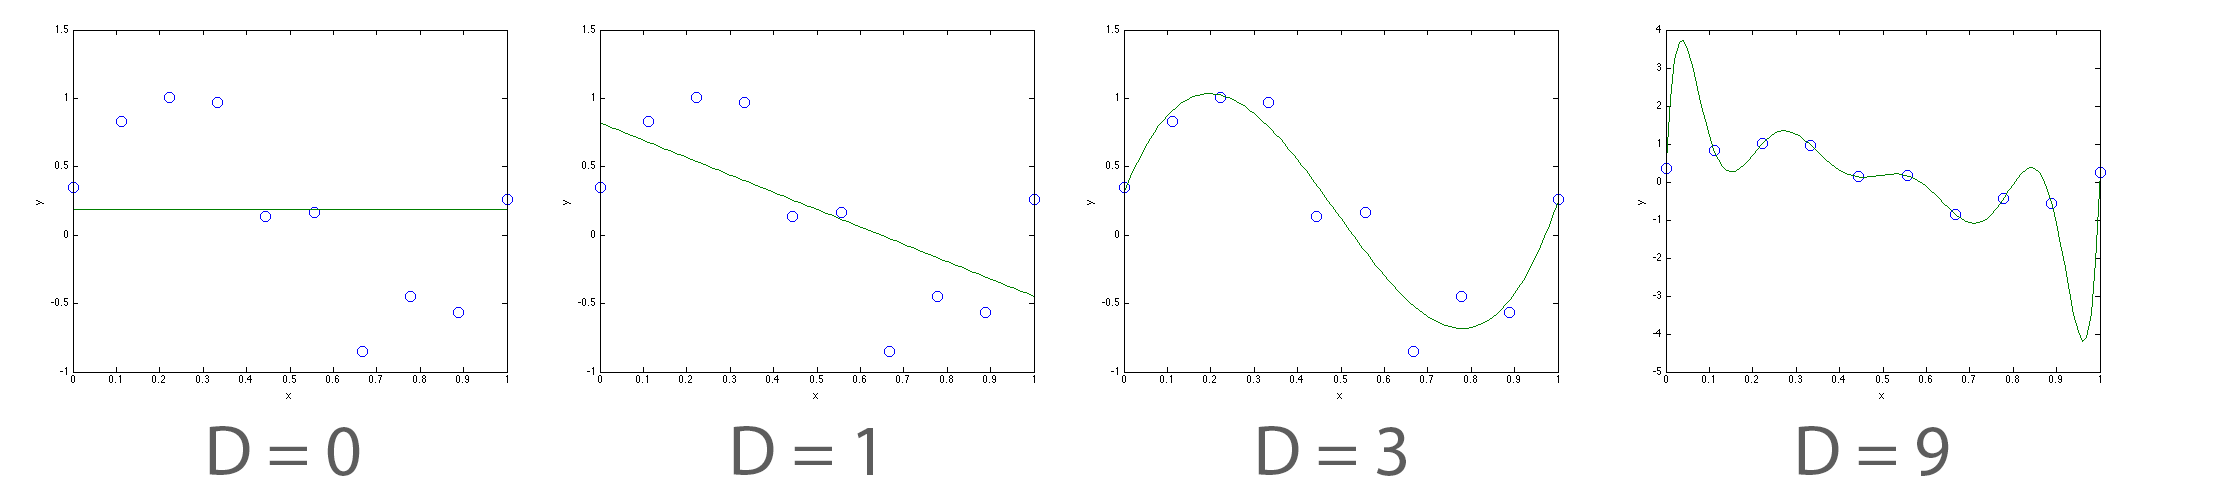
\includegraphics[width=1.0\textwidth]{figures/problem_2_1_full.png}
\end{figure}

\subsection{Gradient Descent}
The other approach is to optimize $W$ by gradient descent. We use the derivative of the error function in order to find a local minimum that satisfies a convergence threshold. For this data set, we use the \textbf{$\overrightarrow{0}$} vector as our initial guess. We use a step size of 0.01 as a parameter to gradient descent. Smaller step sizes take too long to converge and do not improve the final result, while larger step sizes ($> 0.1$) will sometimes never find a solution. A convergence threshold of $10^{-6}$ seems to work well, and it takes around $200$ iterations for the gradient descent algorithm to converge. \\
\\
\indent As expected, the gradient descent method takes significantly longer to run than the analytic solution. The gradient descent method is anywhere from 3 times as slow to 100 times as slow as the exact solution. \textbf{XXX add comparison to matlab optimizers} \\
\\
\begin{figure}[h!]\label{fig-gradient}
  \caption{Gradient descent solution for the linear regress problem with an initial guess of \textbf{0}, a step size of 0.01 and a convergence threshold of $10^{-6}$.}
  \centering
    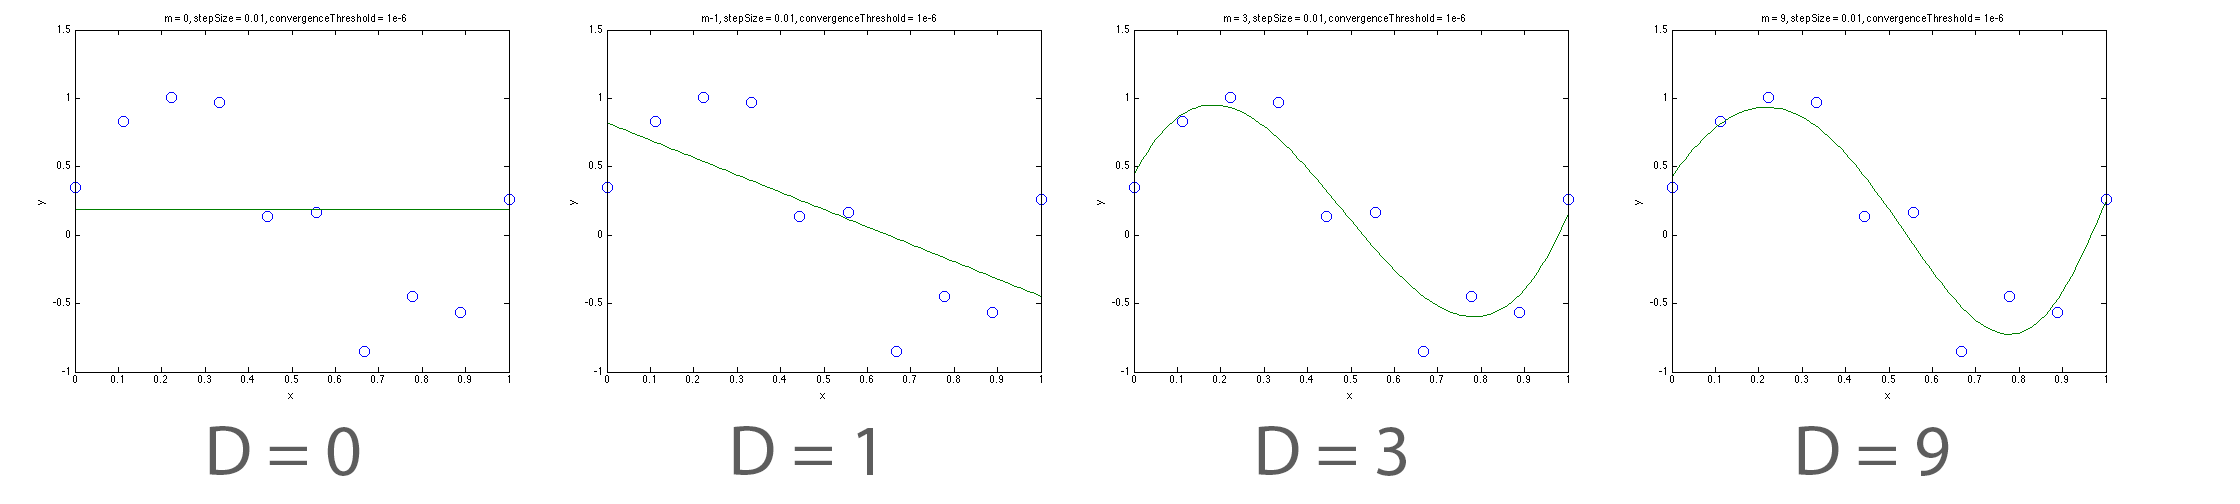
\includegraphics[width=1.0\textwidth]{figures/problem_2_2_full.png}
\end{figure}

\indent Figure~\ref{fig-gradient} shows the results of the gradient descent algorithm with our chosen parameters. The resulting $W$ vector produces a similar curve as the analytic solution for small values of $D$ but starts to diverge from the optimal $W$ as $D$ grows larger. Whereas the analytic solution for $D=9$ fits strongly to the data, the gradient descent solution does not manage to find the global optimum. It is likely that the gradient descent solution gets stuck in a local minimum that is not as optimal as the analytic solution.

\section{Ridge Regression}\label{sec-ridge}

In order to avoid over-fitting, we introduce a parameter $\lambda$ which governs the bias/variance trade-off. Larger values of $\lambda$ introduce bias and reduce variance by decreasing the norm of the weight vector. Another way to view ridge regression is to observe that we are minimizing the same error function with a constraint on the norm of the weight vector. \\
\\
\indent Solving analytically in the same way as Equation~\ref{eq-analytic}, the solution for the weight vector which minimizes error becomes:
\begin{equation}
W_{ridge} = (\textbf{Z}^\textnormal{T}\textbf{Z}+\lambda \textbf{I})^{-1} \textbf{Z}^\textnormal{T} Y_c,
\end{equation}
where $\textbf{Z}$ is a ``centered" data matrix ($z_j^{(i)} = x_j^{(i)} - \bar{x}_j$), and $Y_c$ is a ``centered" version of $Y$ where the mean of all values is 0. \\
\\
\indent

\subsection{Implementation}

\begin{figure}[h!]\label{fig-ridge-bishop}
  \caption{Bishop data set with various feature sets and lambda values.}
  \centering
    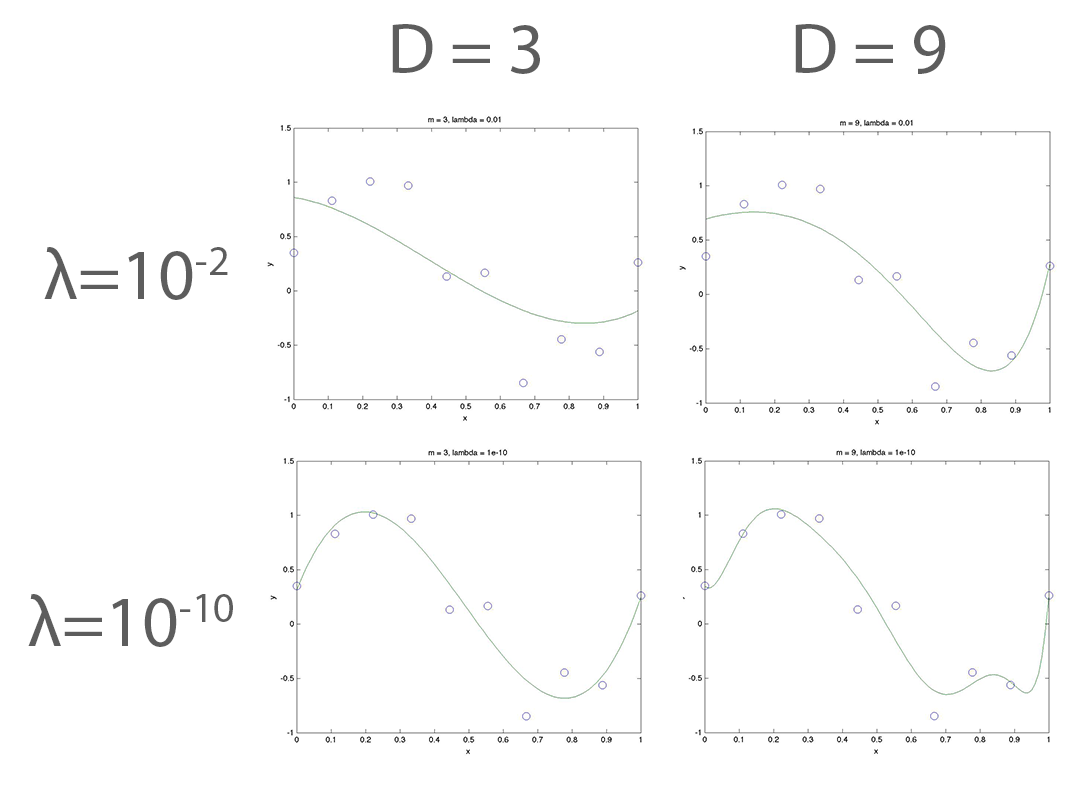
\includegraphics[width=0.5\textwidth]{figures/problem_2_3_bishop.png}
\end{figure}

Ridge regression was implemented and tested on the same data set as in Section~\ref{sec-basis}. Figure~\ref{fig-ridge-bishop} shows the results for various feature sets and lambda values. Higher values of lambda prevented over-fitting but also increased the observed sum-squared error. For $D = 9$ introducing the $\lambda$ parameter definitely improved the solution.

\subsection{Model Selection}

\begin{figure}[h!]\label{fig-training}
  \caption{Training parameters for data set B. On the left, we choose the feature space that minimizes validation error. On the right, we choose a value of lambda that minimizes validation error. }
  \centering
    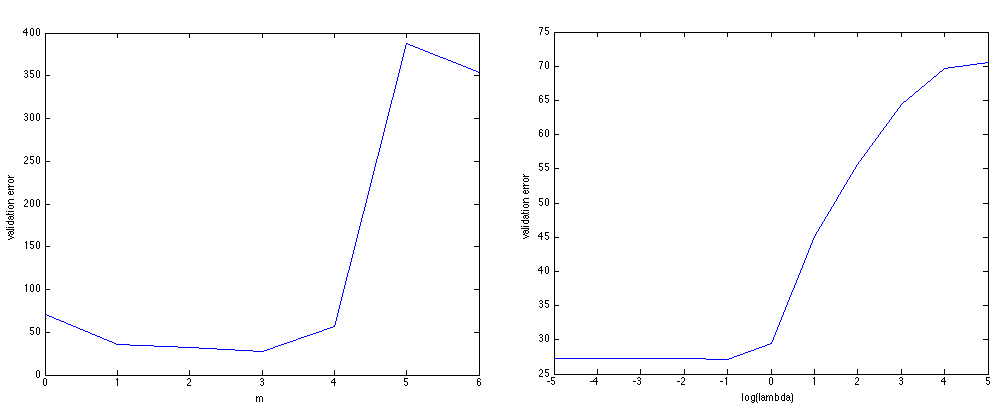
\includegraphics[width=0.5\textwidth]{figures/3_2_training.png}
\end{figure}

\begin{figure}[h!]\label{fig-result}
  \caption{ Solution  for data set B with approximately optimal parameters in both the training data set (left) and validation data set (right). }
  \centering
    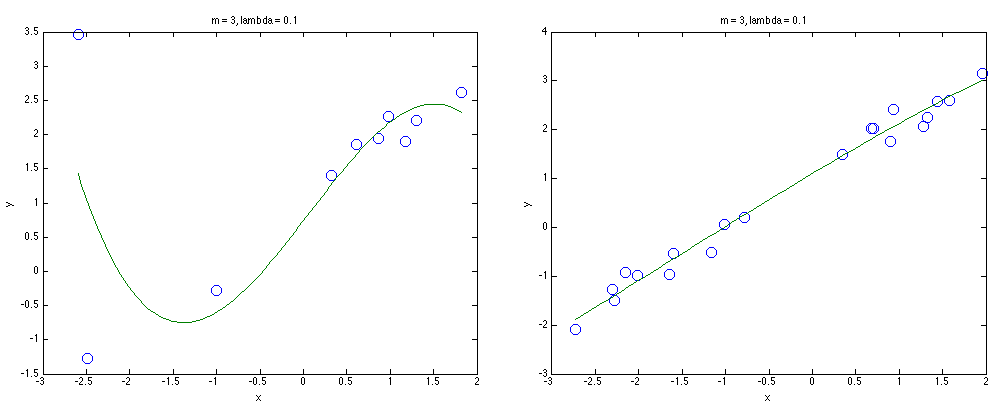
\includegraphics[width=0.5\textwidth]{figures/3_2_result.png}
\end{figure}

In order to accurately model the data, we have to systematically choose parameters that satisfy previously unseen data. In this case, we were given two ``training" data sets and one ``validation" set. To determine the optimal parameters, we loop through a variety of feature spaces and $\lambda$ values. For each pair of values, we determine our weight vector $W$ from the training data set and then measure its performance on the validation data set. Figure~\ref{fig-training} shows the validation error on data set B for a variety of feature sizes and lambda values, and Figure~\ref{fig-result} shows the resulting weight vector that optimized validation performance. We found that $D=3, \lambda=0.1$ produced the best solution for data set B, and $D=1,\lambda=0$ produced the best solution for data set A.
\subsection{Real World Data}
\begin{figure}[h!]\label{fig-blog}
  \caption{ Optimizing $\lambda$ for the blog data set. }
  \centering
    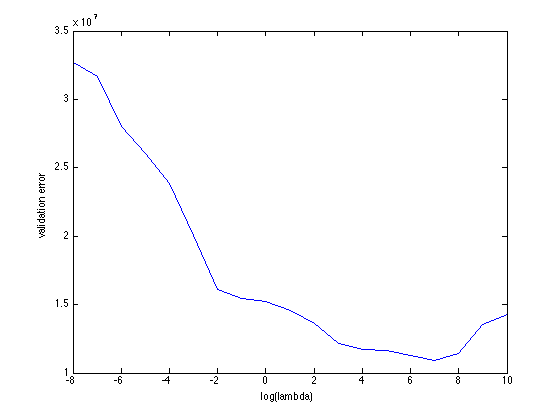
\includegraphics[width=0.5\textwidth]{figures/3_3_choosing_lambda.png}
\end{figure}

We were also given a real world data which mapped blog feedback rates to various environmental parameters. We used a simple linear model for this case and used the training/validation data sets to determine an optimal $\lambda$ parameter. We tested $\lambda$ values from $10^{-7}$ to $10^{10}$ and observed that a $\lambda$ value of approximately $10^7$ minimized validation error (see Figure~\ref{fig-blog}).
\end{document}
